\chapter{CÀI ĐẶT VÀ ĐÁNH GIÁ KẾT QUẢ}
\section{Mô tả dữ liệu}
%chèn plot giá của tập dữ liệu theo thời gian, nêu rõ thời gian thu thập, nguồn thu thập, kích thước dữ liệu, tỉ lệ chia tập train, val, test
Để thực hiện dự đoán trên hai mô hình LSTM và VARMAX, chúng em sẽ thực nghiệm trên dữ liệu về chỉ số môi trường không khí.
\begin{itemize}
    \item Nguồn thu thập: Được cung cấp bởi giảng viên bộ môn
    \item Thời gian của dữ liệu: 142 ngày từ 7:00 14/4/2019 đến 6:00 5/9/2019 tính theo từng giờ.
    \item Kích thước dữ liệu: 556KB
    \item Giá trị cần dự đoán: mô hình dự đoán tất cả các giá trị trong bộ dữ liệu
    
\end{itemize}
\begin{figure}[H]
    \centering
    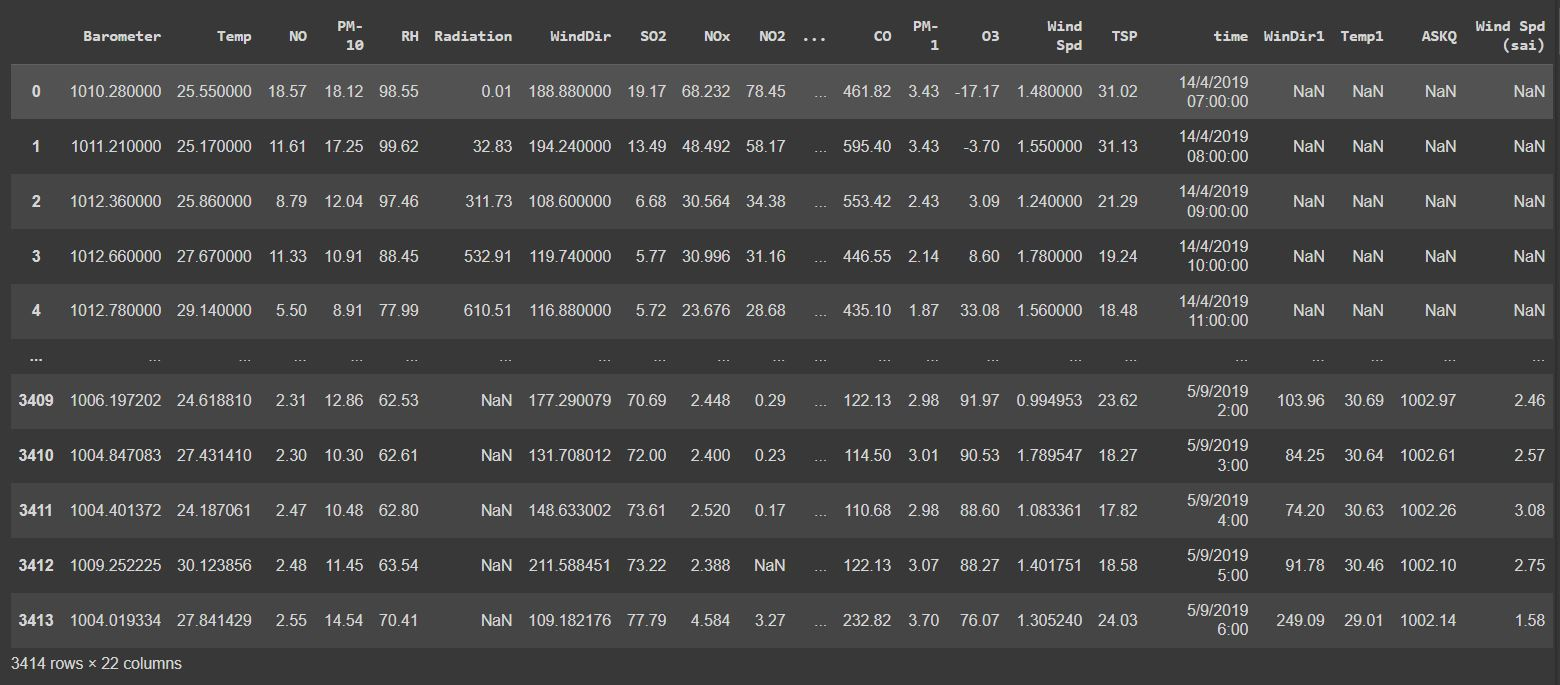
\includegraphics[width=.95\textwidth]{figures/data.jpg}
    \caption[Dữ liệu môi trường không khí từ  7:00 14/4/2019 đến 6:00 5/9/2019]{Dữ liệu môi trường không khí từ  7:00 14/4/2019 đến 6:00 5/9/2019}
\end{figure}


Mô tả chi tiết tên các cột :
\begin{itemize}
    \item Barometer: hay còn được gọi với thuật ngữ quen thuộc là áp kế, là tính năng dùng để đo áp suất khí quyển ở vị trí hiện tại của đồng hồ. Đơn vị đo áp suất phổ biến hiện nay là (hPa) = hectopascal, ngoài ra còn 2 đơn vị được sử dụng nhiều là kilopascal (kPa) và atmosphere (atm).
    \item Temp : là nhiệt độ đơn vị độ C
    \item NO : Nitơ monoxide, hay còn gọi là nitric oxide (công thức hóa học: NO) là chất khí không màu, không bền trong không khí vì bị oxy oxy hóa ở nhiệt độ thường tạo ra nitơ dioxide là chất khí màu nâu đỏ. NO được tạo ra từ năng lượng sấm sét
    \item NO2 : Nitrogen dioxide (NO 2 ) là một chất góp phần chính trong việc hình thành sương mù và là tiền thân của nhiều chất ô nhiễm thứ cấp có hại, bao gồm ozone và các chất dạng hạt. Nó phản ứng mạnh với các hóa chất khác và là một chất oxy hóa mạnh. Nitơ đioxit là một chất khí có màu đỏ cam đậm.
    \item NOx : là chất gây ô nhiễm chính trong khí quyển, là tác nhân của mưa axit, sương khói quang hóa và tích tụ ozone. Các oxit chủ yếu là nitơ monoxit (NO) và nitơ dioxit (NO2) cả hai đều ăn mòn và nguy hiểm cho sức khỏe.
    \item PM-10 : PM-10 là những hạt rất nhỏ được tìm thấy trong bụi và khói . Chúng có đường kính 10 micromet (0,01 mm) hoặc nhỏ hơn. Các hạt PM-10 là một chất gây ô nhiễm không khí phổ biến.
    \item RH : Độ ẩm tương đối (RH) là thước đo lượng hơi nước trong hỗn hợp nước-không khí so với lượng tối đa có thể. RH là tỷ lệ giữa tỷ lệ độ ẩm của hỗn hợp nước-không khí cụ thể so với tỷ lệ độ ẩm bão hòa ở một nhiệt độ nhất định.
    \item Radition : Bức xạ khí quyển là dòng năng lượng điện từ giữa mặt trời và bề mặt trái đất khi nó bị ảnh hưởng bởi các đám mây và khí trong bầu khí quyển của trái đất. Nó bao gồm cả bức xạ mặt trời (ánh sáng mặt trời) và bức xạ nhiệt.
    \item SO2 : Lưu huỳnh dioxit là chất gây ô nhiễm không khí phản ứng, không màu, có mùi nồng . Loại khí này có thể là mối đe dọa đối với sức khỏe con người, sức khỏe động vật và đời sống thực vật. Các nguồn phát thải sulfur dioxide chính là từ quá trình đốt cháy nhiên liệu hóa thạch và hoạt động núi lửa tự nhiên.
    \item PM-2-5: là những hạt bụi li ti có trong không khí với kích thước 2,5 micron trở xuống (so với sợi tóc con người thì nó nhỏ hơn khoảng 30 lần). Bụi mịn pm2. 5 được hình thành từ các chất như nitơ, carbon và các hợp chất kim loại khác. Nó chất gây ô nhiễm không khí gây lo ngại cho sức khỏe của mọi người khi nồng độ trong không khí cao.
    \item CO: Cacbon monoxit là một chất khí vô hình, không hề có màu sắc, vô vị, không hề có mùi, và nó là một chất độc nguy hiểm với độc tính cao. Nó là sản phẩm chính của quá trình đốt cháy nhiên liệu trong môi trường không đủ oxy.
    \item Là những hạt bụi dạng lỏng, hoặc rắn trôi nổi ngoài không khí. PM1 được coi là đặc biệt nguy hiểm do kích thước cực nhỏ của nó. Đường kính của hạt càng nhỏ thì nó càng gây ra nhiều tác hại.
    \item O3 : là một chất khí màu xanh lam nhạt, có mùi hăng đặc biệt. Nó là một dạng thù hình của oxy kém bền hơn nhiều so với dạng nguyên tử O2, bị phá vỡ trong bầu khí quyển thấp hơn thành O2.
    \item Wind Spd : Tốc độ gió hay còn gọi là tốc độ luồng gió, là một đại lượng khí quyển cơ bản do không khí di chuyển từ nơi có áp suất cao đến áp suất thấp.
    \item TSP: Tổng bụi lơ lửng (TSP) là tổng các hạt bụi có đường kính khí động học nhỏ hơn hoặc bằng 100 micromet. 
\end{itemize}

\newpage
\section{Xử lý dữ liệu}
\noindent \textbf{Vấn đề của bộ dữ liệu} : có khá nhiều dữ liệu bị khuyết thiếu.
\begin{figure}[H]
    \centering
    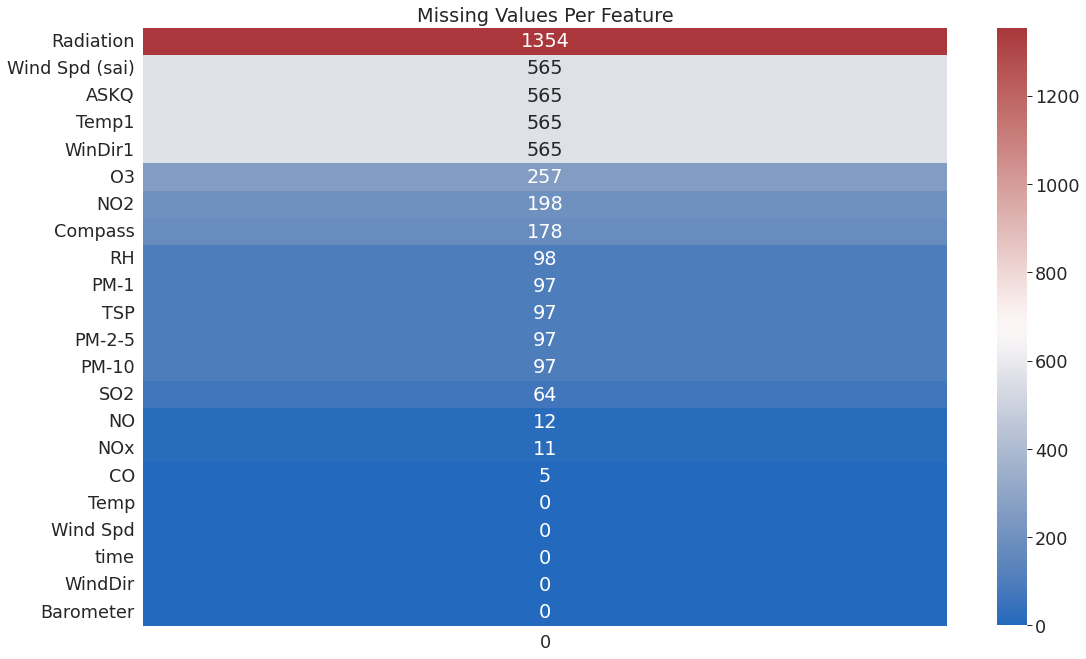
\includegraphics[width=.93\textwidth]{figures/missing.png}
    \caption[Số lượng dữ liệu khuyết thiếu của từng cột]{Số lượng dữ  liệu khuyết thiếu của từng cột}
\end{figure}

\begin{figure}[H]
    \centering
    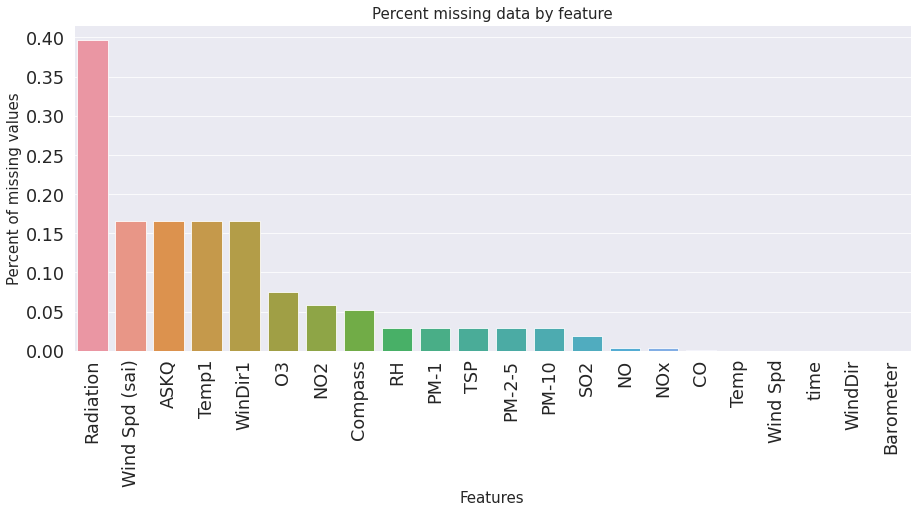
\includegraphics[width=.95\textwidth]{figures/missing2.png}
    \caption[Tỷ lệ dữ liệu khuyết thiếu của từng cột]{Tỷ lệ dữ liệu khuyết thiếu của từng cột}
\end{figure}

Nhận thấy tỷ lệ dữ liệu khuyết thiếu của từng cột cũng không cao lắm nên có thể giữ lại và sẽ sử dụng Linear-Regression để dự đoán các giá trị còn thiếu như sau:
\begin{lstlisting}
from sklearn.linear_model import LinearRegression
linreg = LinearRegression()

lst = ['CO', 'NOx','NO','SO2','PM-10','PM-2-5','TSP','PM-1','RH','Compass', 'NO2','O3','WinDir1','Temp1','ASKQ','Wind Spd (sai)','Radiation']
data = df[['Barometer','Wind Spd','Temp','WindDir']]
for a in lst:
    data = pd.concat([data, df[a]], axis=1)
    x_train = data[data[a].notnull()].drop(columns=a)
    y_train = data[data[a].notnull()][a]
    x_test = data[data[a].isnull()].drop(columns=a)
    y_test = data[data[a].isnull()][a]
    linreg.fit(x_train, y_train)
    predicted = linreg.predict(x_test)
    data[a][data[a].isnull()] = predicted
    df[a][df[a].isnull()] = predicted
    print("done")
\end{lstlisting}

\noindent Trong đó:
\begin{itemize}
    \item \textbf{lst} là 1 mảng chứa tên các cột bị thiếu dữ liệu được sắp xếp theo số lượng tăng dần.
    \item \textbf{data} chứa các cột có đủ dữ liệu.
\end{itemize}

\noindent Thực hiện:
\begin{itemize}
    \item Ta sử dụng vòng lặp for để dự đoán các cột có số lượng dữ liệu bị thiếu ít hơn trước. 
    \item Trong vòng lặp for, ta thêm 1 cột khuyết thiếu dữ liệu vào \textbf{data}
    \item Chia dữ liệu thành tập train và test:
    \begin{itemize}
        \item train: chứa các dòng dữ liệu đầy đủ.
        \item test: chứa các dòng dữ liệu bị khuyết thiếu.
    \end{itemize}
    \item Sử dụng mô hình dự đoán Linear-Regression để đưa ra kết quả dự đoán của tập test và tiếp tục quá trình nếu còn thỏa mãn vòng lặp.
\end{itemize}
\newpage
\noindent Kết quả thu được:
\begin{figure}[H]
    \centering
    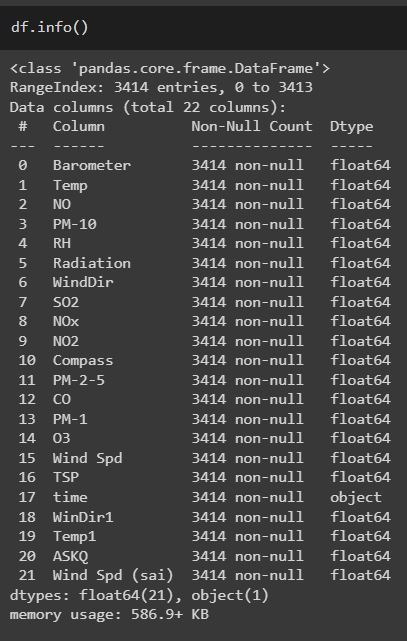
\includegraphics[width=.3\textwidth]{figures/info.jpg}
    \caption[Thông tin dữ liệu sau khi xử lý]{Thông tin dữ liệu sau khi xử lý}
\end{figure}

\begin{figure}[H]
    \centering
    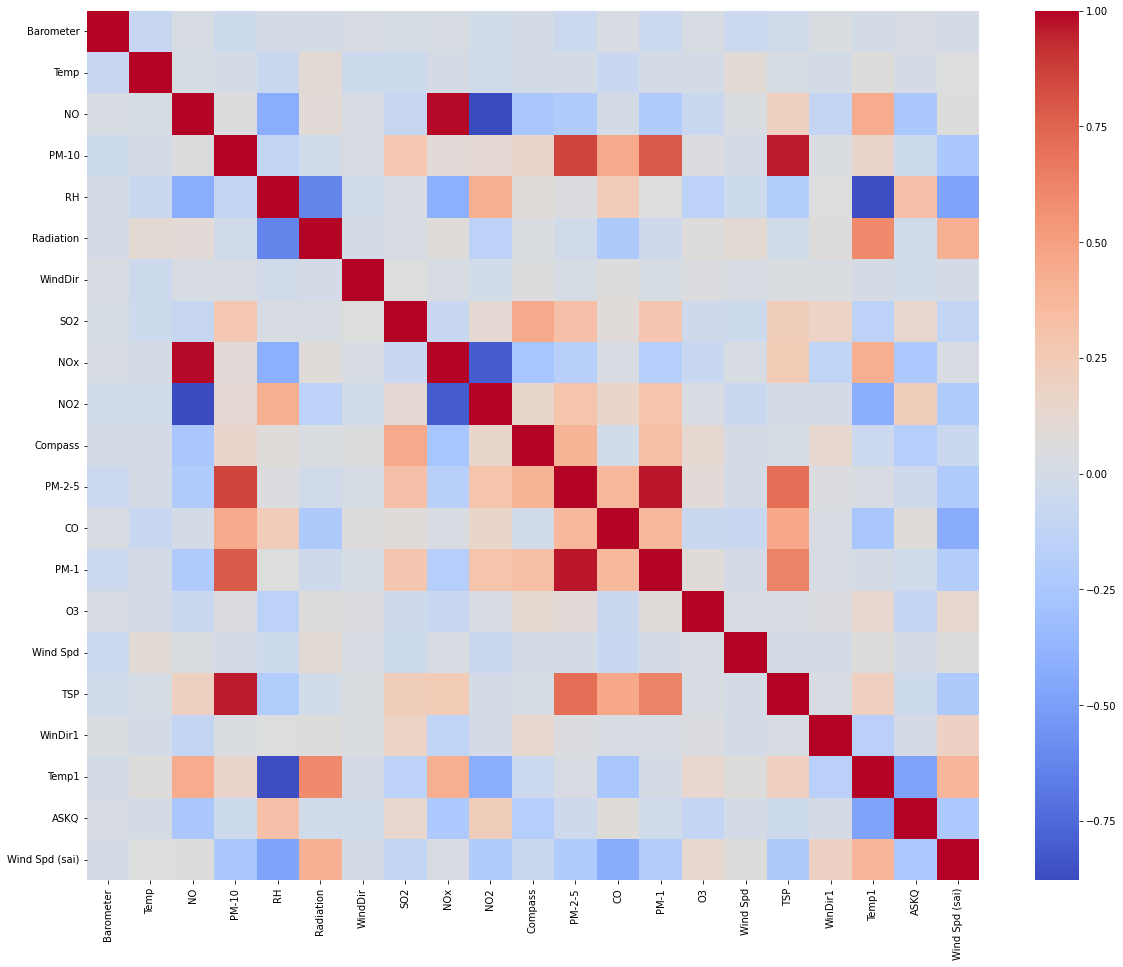
\includegraphics[width=.9\textwidth]{figures/matran.png}
    \caption[Heatmap]{Heatmap}
\end{figure}

\newpage
\begin{figure}[H]
    \centering
    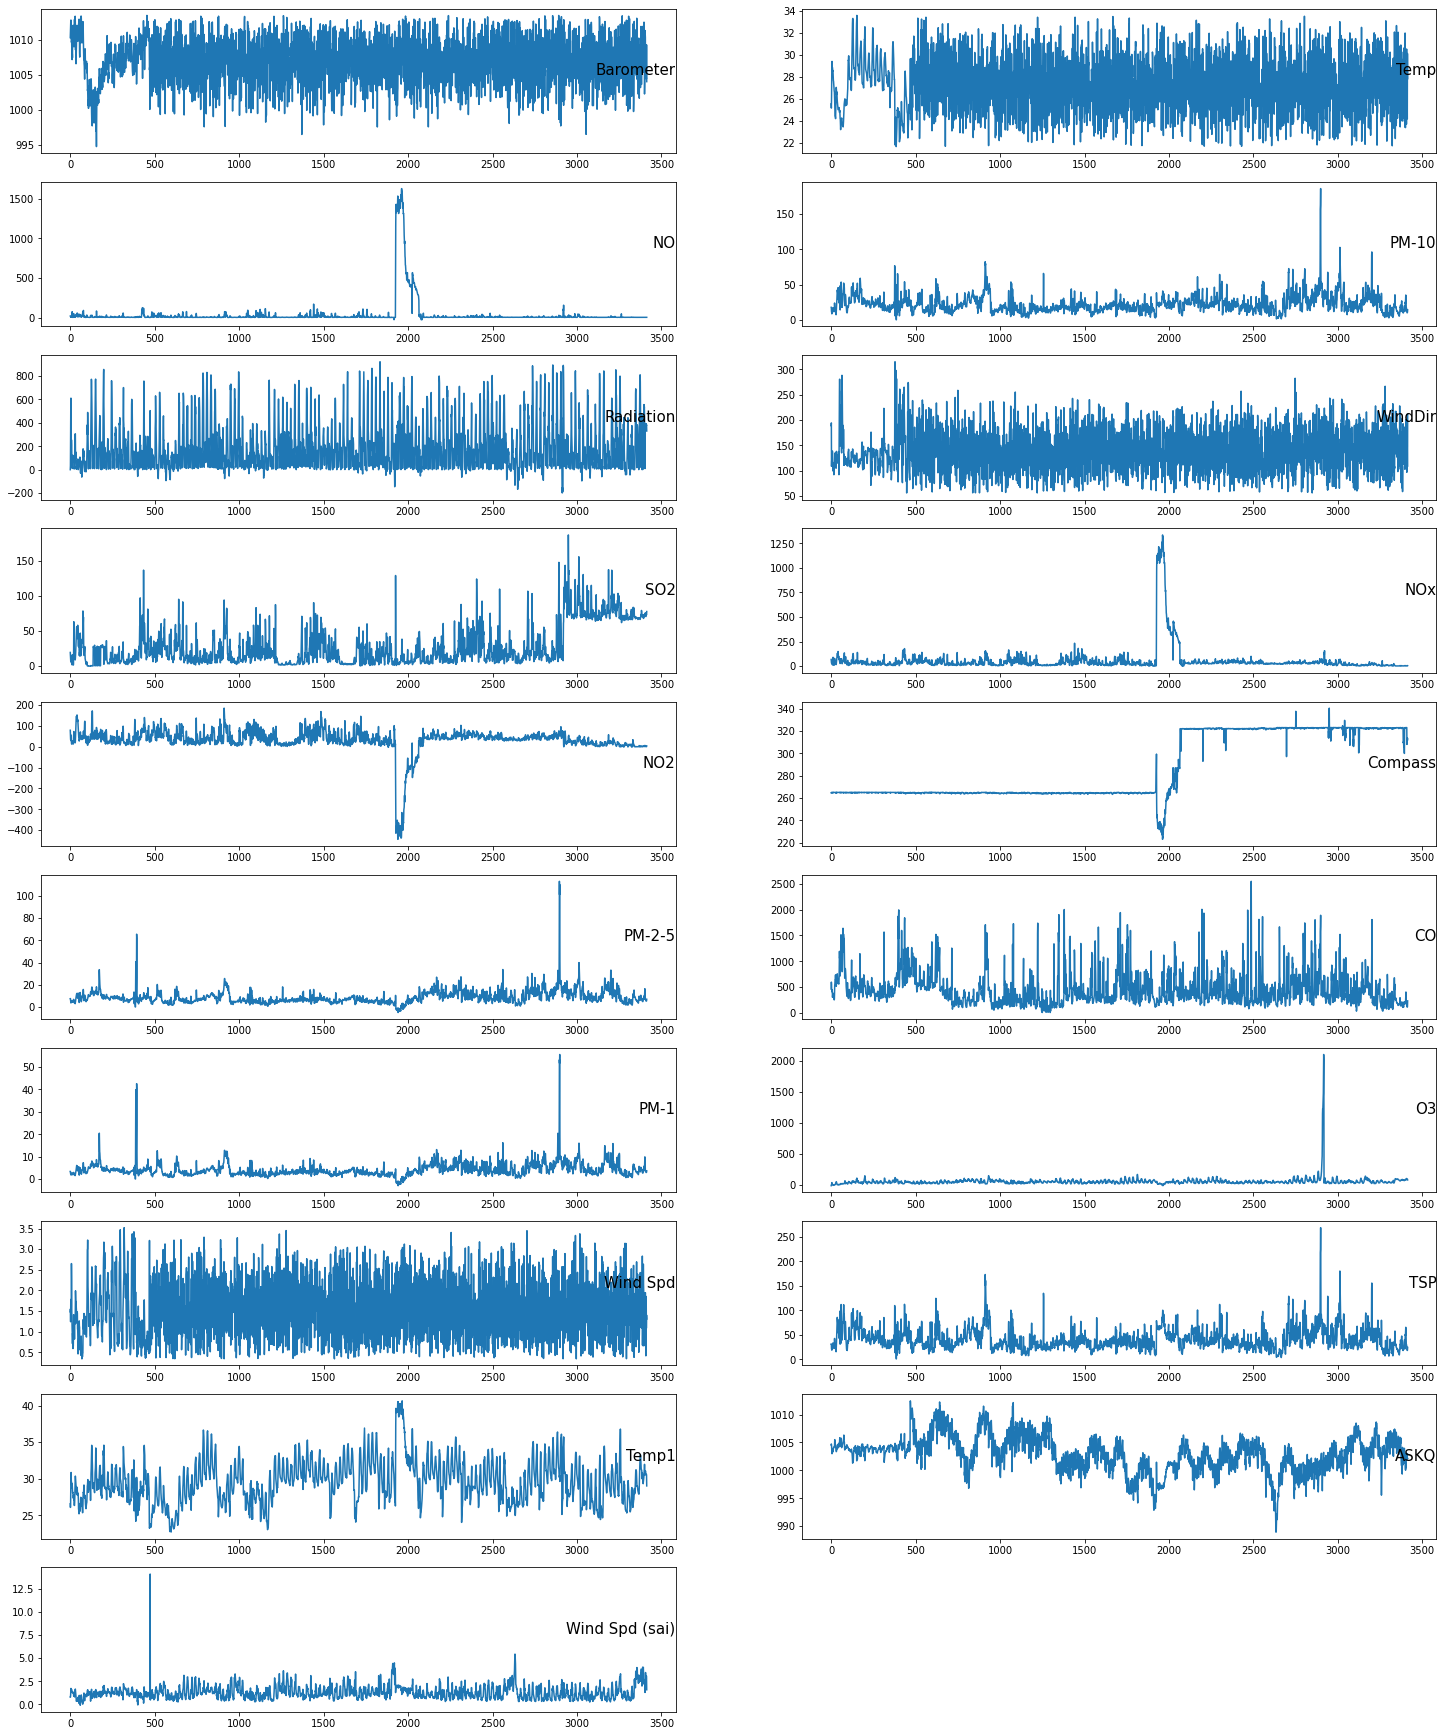
\includegraphics[width=.99\textwidth]{figures/trucquan.png}
    \caption[Trực quan hóa dữ liệu]{Trực quan hóa dữ liệu}
\end{figure}

\section{Tiêu chuẩn đánh giá mô hình}
%RMSE, MAE, MAPE
\subsection{Mean Squared Error (MSE)}
MSE được hiểu là giá trị sai số bình phương trung bình hoặc là lỗi bình phương trung bình. Nó đề cập đến giá trị trung bình của chênh lệch bình phương giữa tham số dự đoán và tham số quan sát được và có công thức như sau:
\begin{equation}
    \text{MSE} = \frac{1}{n}\sum_{i=1}^n(y_i - \hat{y_i})^2
\end{equation}
với $y_i$ là giá trị thực sự cần dự đoán, và $\hat{y}_i$ là giá trị mô hình dự đoán, $n$ là kích thước của dữ liệu cần dự đoán.


\subsection{Root Mean Squared Error (RMSE)}
RMSE là thước đo mức độ hiệu quả của mô hình của bạn. Nó thực hiện điều này bằng cách đo sự khác biệt giữa các giá trị dự đoán và giá trị thực tế . R-MSE càng nhỏ tức là sai số càng bé thì mức độ ước lượng cho thấy độ tin cậy của mô hình có thể đạt cao nhất và có công thức tính là:
\begin{equation}
    \text{RMSE} = \sqrt{\frac{1}{n}\sum_{i=1}^n(y_i - \hat{y_i})^2}
\end{equation}
với $y_i$ là giá trị thực sự cần dự đoán, và $\hat{y}_i$ là giá trị mô hình dự đoán, $n$ là kích thước của dữ liệu cần dự đoán.

\subsection{Sử dụng \textit{model.plot\_diagnostics()}}
\noindent Tạo lưới ô 2x2 chứa các kết quả đánh giá mô hình:
\begin{enumerate}
    \item Standardized residuals 
    \item Histogram plus estimated density 
    \item Normal Q-Q
    \item Correlogram
\end{enumerate}

\section{Kết quả}
%chèn plot so sánh kết quả ở tập train, tập test.
%ghi kết quả vào bảng sau
\subsection{Mô hình LSTM}
Đánh giá mô hình :
\begin{itemize}
    \item Loss: được tính bằng MSE, LOSS của mô hình sau khi huấn luyện qua 200 epoch
    \begin{figure}[H]
    \centering
    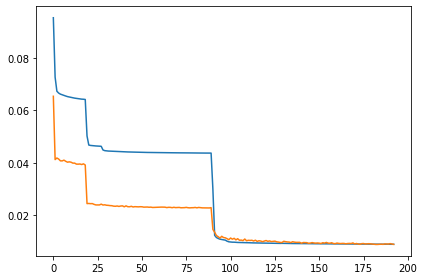
\includegraphics[width=.95\textwidth]{figures/LOSS_LSTM.png}
    \caption[LOSS của mô hình LSTM]{LOSS của mô hình LSTM}
    \end{figure}
    \item RMSE của mô hình sau khi huấn luyện qua 200 epoch:
    \begin{figure}[H]
    \centering
    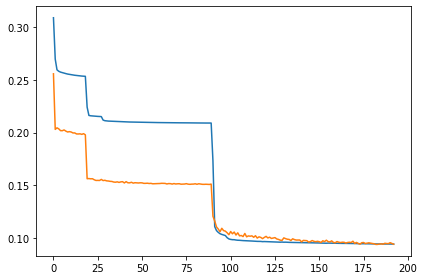
\includegraphics[width=.95\textwidth]{figures/RMSE_LSTM.png}
    \caption[RMSE của mô hình LSTM]{RMSE của mô hình LSTM}
\end{figure}

\end{itemize}
Kết quả dự đoán của mô hình với 48 giờ cuối của bộ dữ liệu so với giá trị thực trên tập dữ liệu:
    \begin{figure}[H]
    \centering
    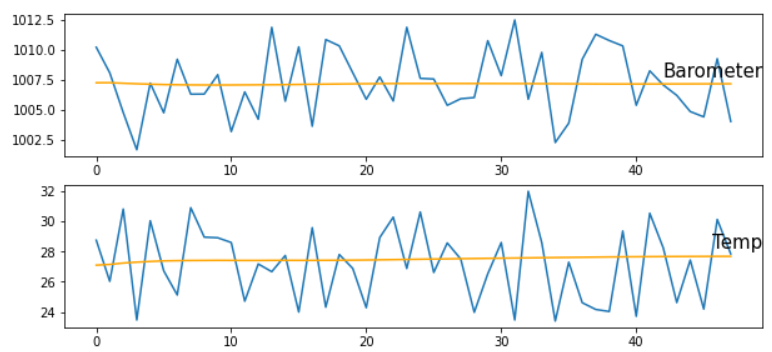
\includegraphics[width=1\textwidth]{figures/LSTM_test1.png}
    \caption[Barometer và Temp]{Barometer và Temp}
\end{figure}
\newpage
\begin{figure}[H]
    \centering
    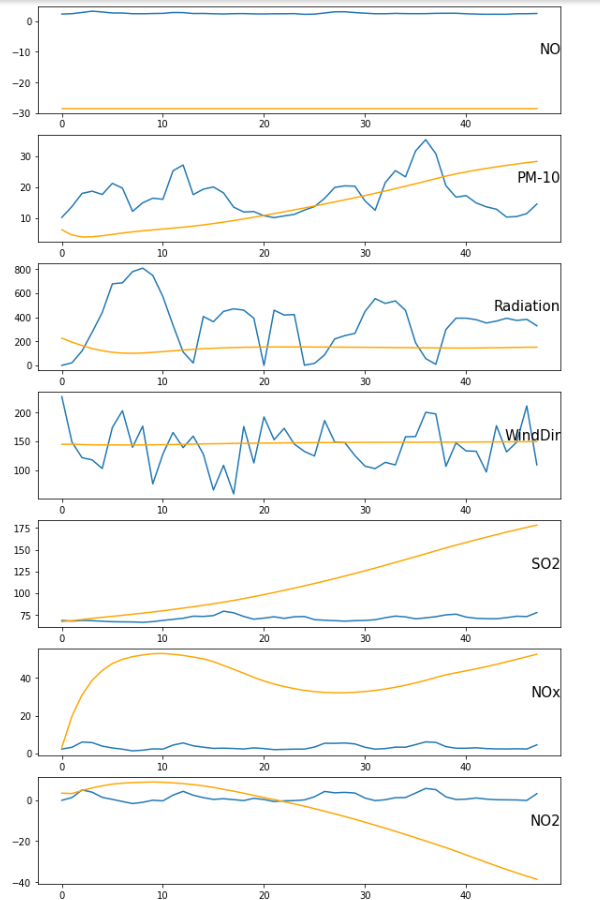
\includegraphics[width=.95\textwidth]{figures/LSTM_test3.png}
    \caption[NO, PM-10, Radition, WindDir và SO2]{NO, PM-10, Radition, WindDir, SO2, NOx và NO2}
\end{figure}
\newpage
\begin{figure}[H]
    \centering
    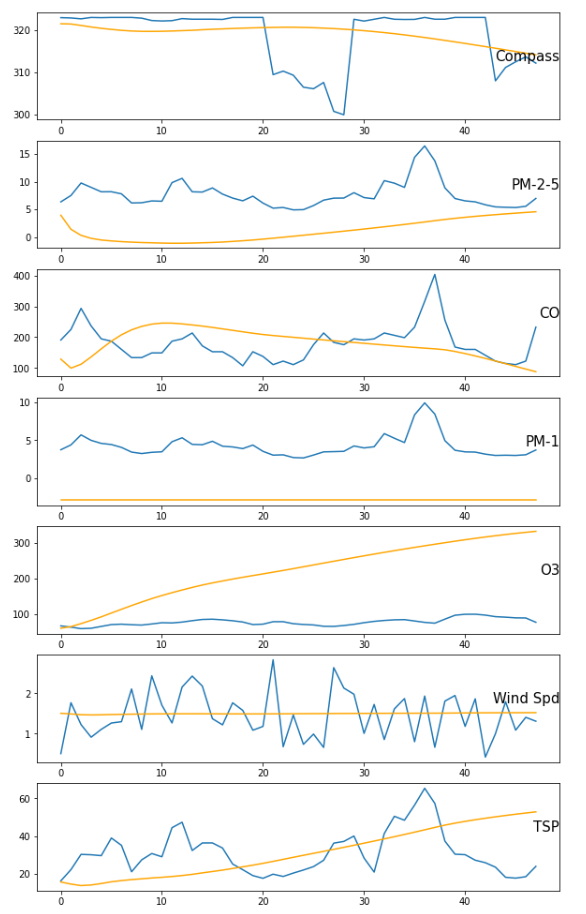
\includegraphics[width=.95\textwidth]{figures/LSTM_test4.png}
    \caption[Compass, PM-2-5, CO, PM-1, O3, Wind Spd và TSP]{Compass, PM-2-5, CO, PM-1, O3, Wind Spd và TSP}
\end{figure}
\newpage
\begin{figure}[H]
    \centering
    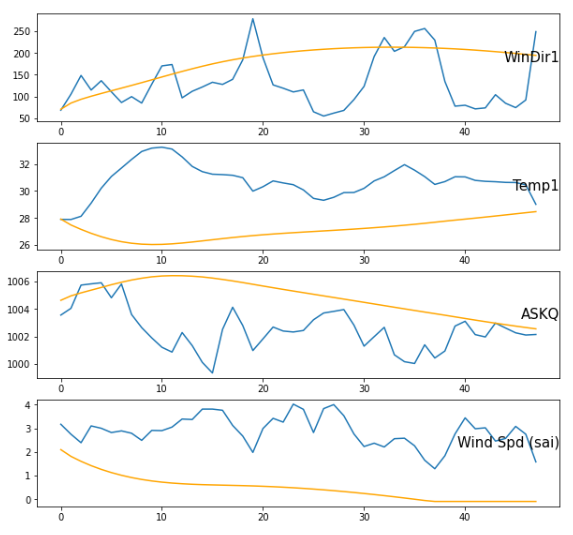
\includegraphics[width=1\textwidth]{figures/LSTM_test5.png}
    \caption[WinDir1, Temp1, ASKQ, Wind-Spd(sai)]{WinDir1, Temp1, ASKQ, Wind-Spd(sai)}
\end{figure}
Nhận xét:
\begin{itemize}
    \item Mô hình LSTM cho MSE và RMSE đều thấp. Sau 200, LOSS giảm dần về 0 và RMSE giảm còn 0.1.
    \item Kết quả dự đoán so với kết quả test không khớp nhau vẫn còn chênh lệch khá nhiều.
    \item Một số cột kết quả dự đoán cho giá trị là một đường thẳng.
    \item Mặc dù cả LOSS và RMSE đều thấp nhưng mô hình dự đoán kết quả lại không tốt.
    \item Mô hình không phù hợp với bộ dữ liệu.
\end{itemize}
\newpage
\subsection{Mô hình VARMAX}
\begin{enumerate}
    \item Đánh giá mô hình:
    \begin{itemize}
    \item Giá trị MSE của mô hình sau khi huấn luyện qua 1000 epoch (maxiter = 1000) là \textbf{1031.6635015800691} 

    \item Kết quả đánh giá theo một số cột:
    \begin{figure}[H]
        \centering
        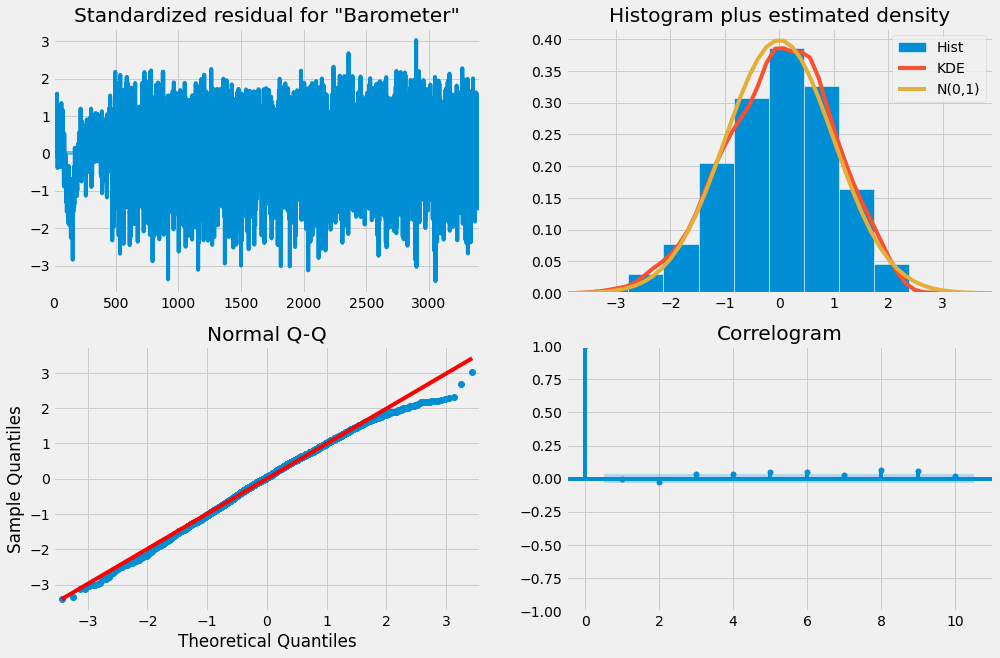
\includegraphics[width=0.75\textwidth]{figures/danhgia1.png}
        \caption[Barometer]{Barometer}
    \end{figure}

    %\begin{figure}[H]
     %   \centering
     %   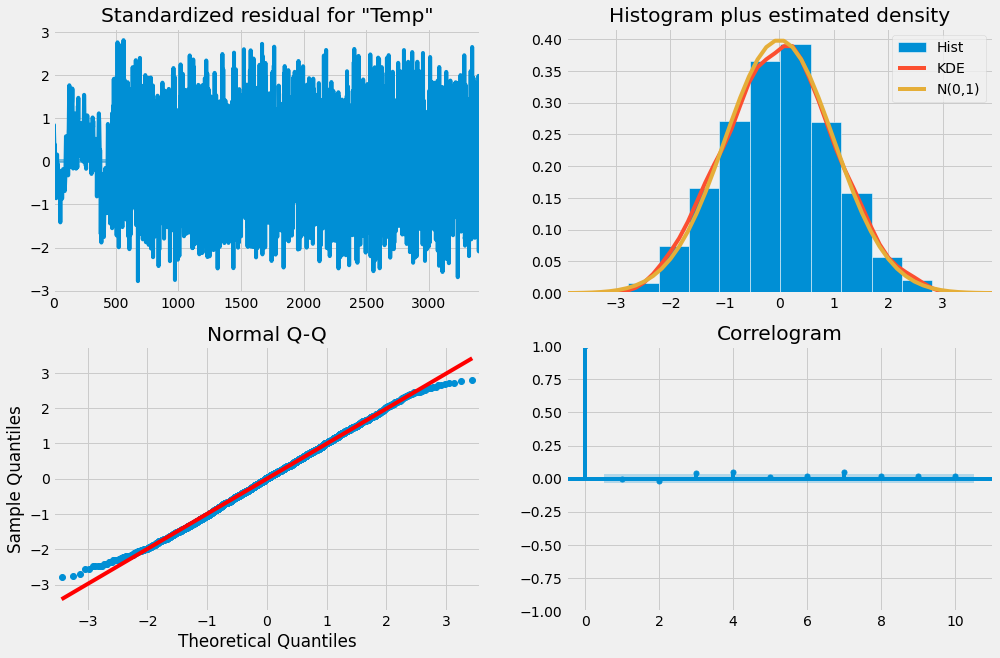
\includegraphics[width=0.7\textwidth]{figures/danhgia.png}
     %   \caption[Temp]{Temp}
    %\end{figure}

    \begin{figure}[H]
        \centering
        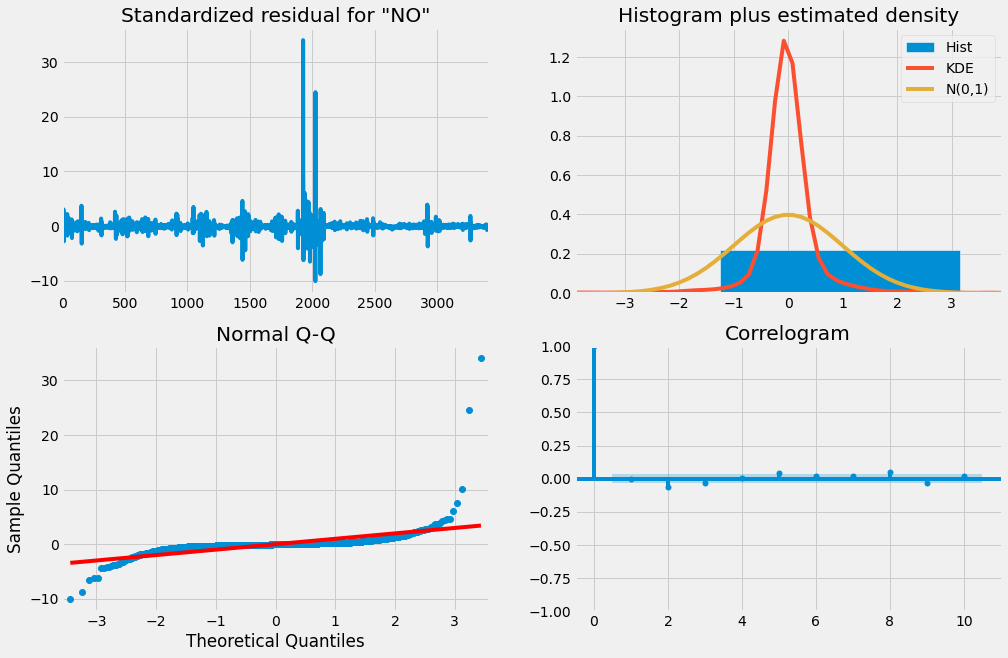
\includegraphics[width=0.75\textwidth]{figures/danhgia3.png}
        \caption[NO]{NO}
    \end{figure}
    
\end{itemize}

    \item Kết quả dự đoán so với tập test
    \begin{figure}[H]
        \centering
        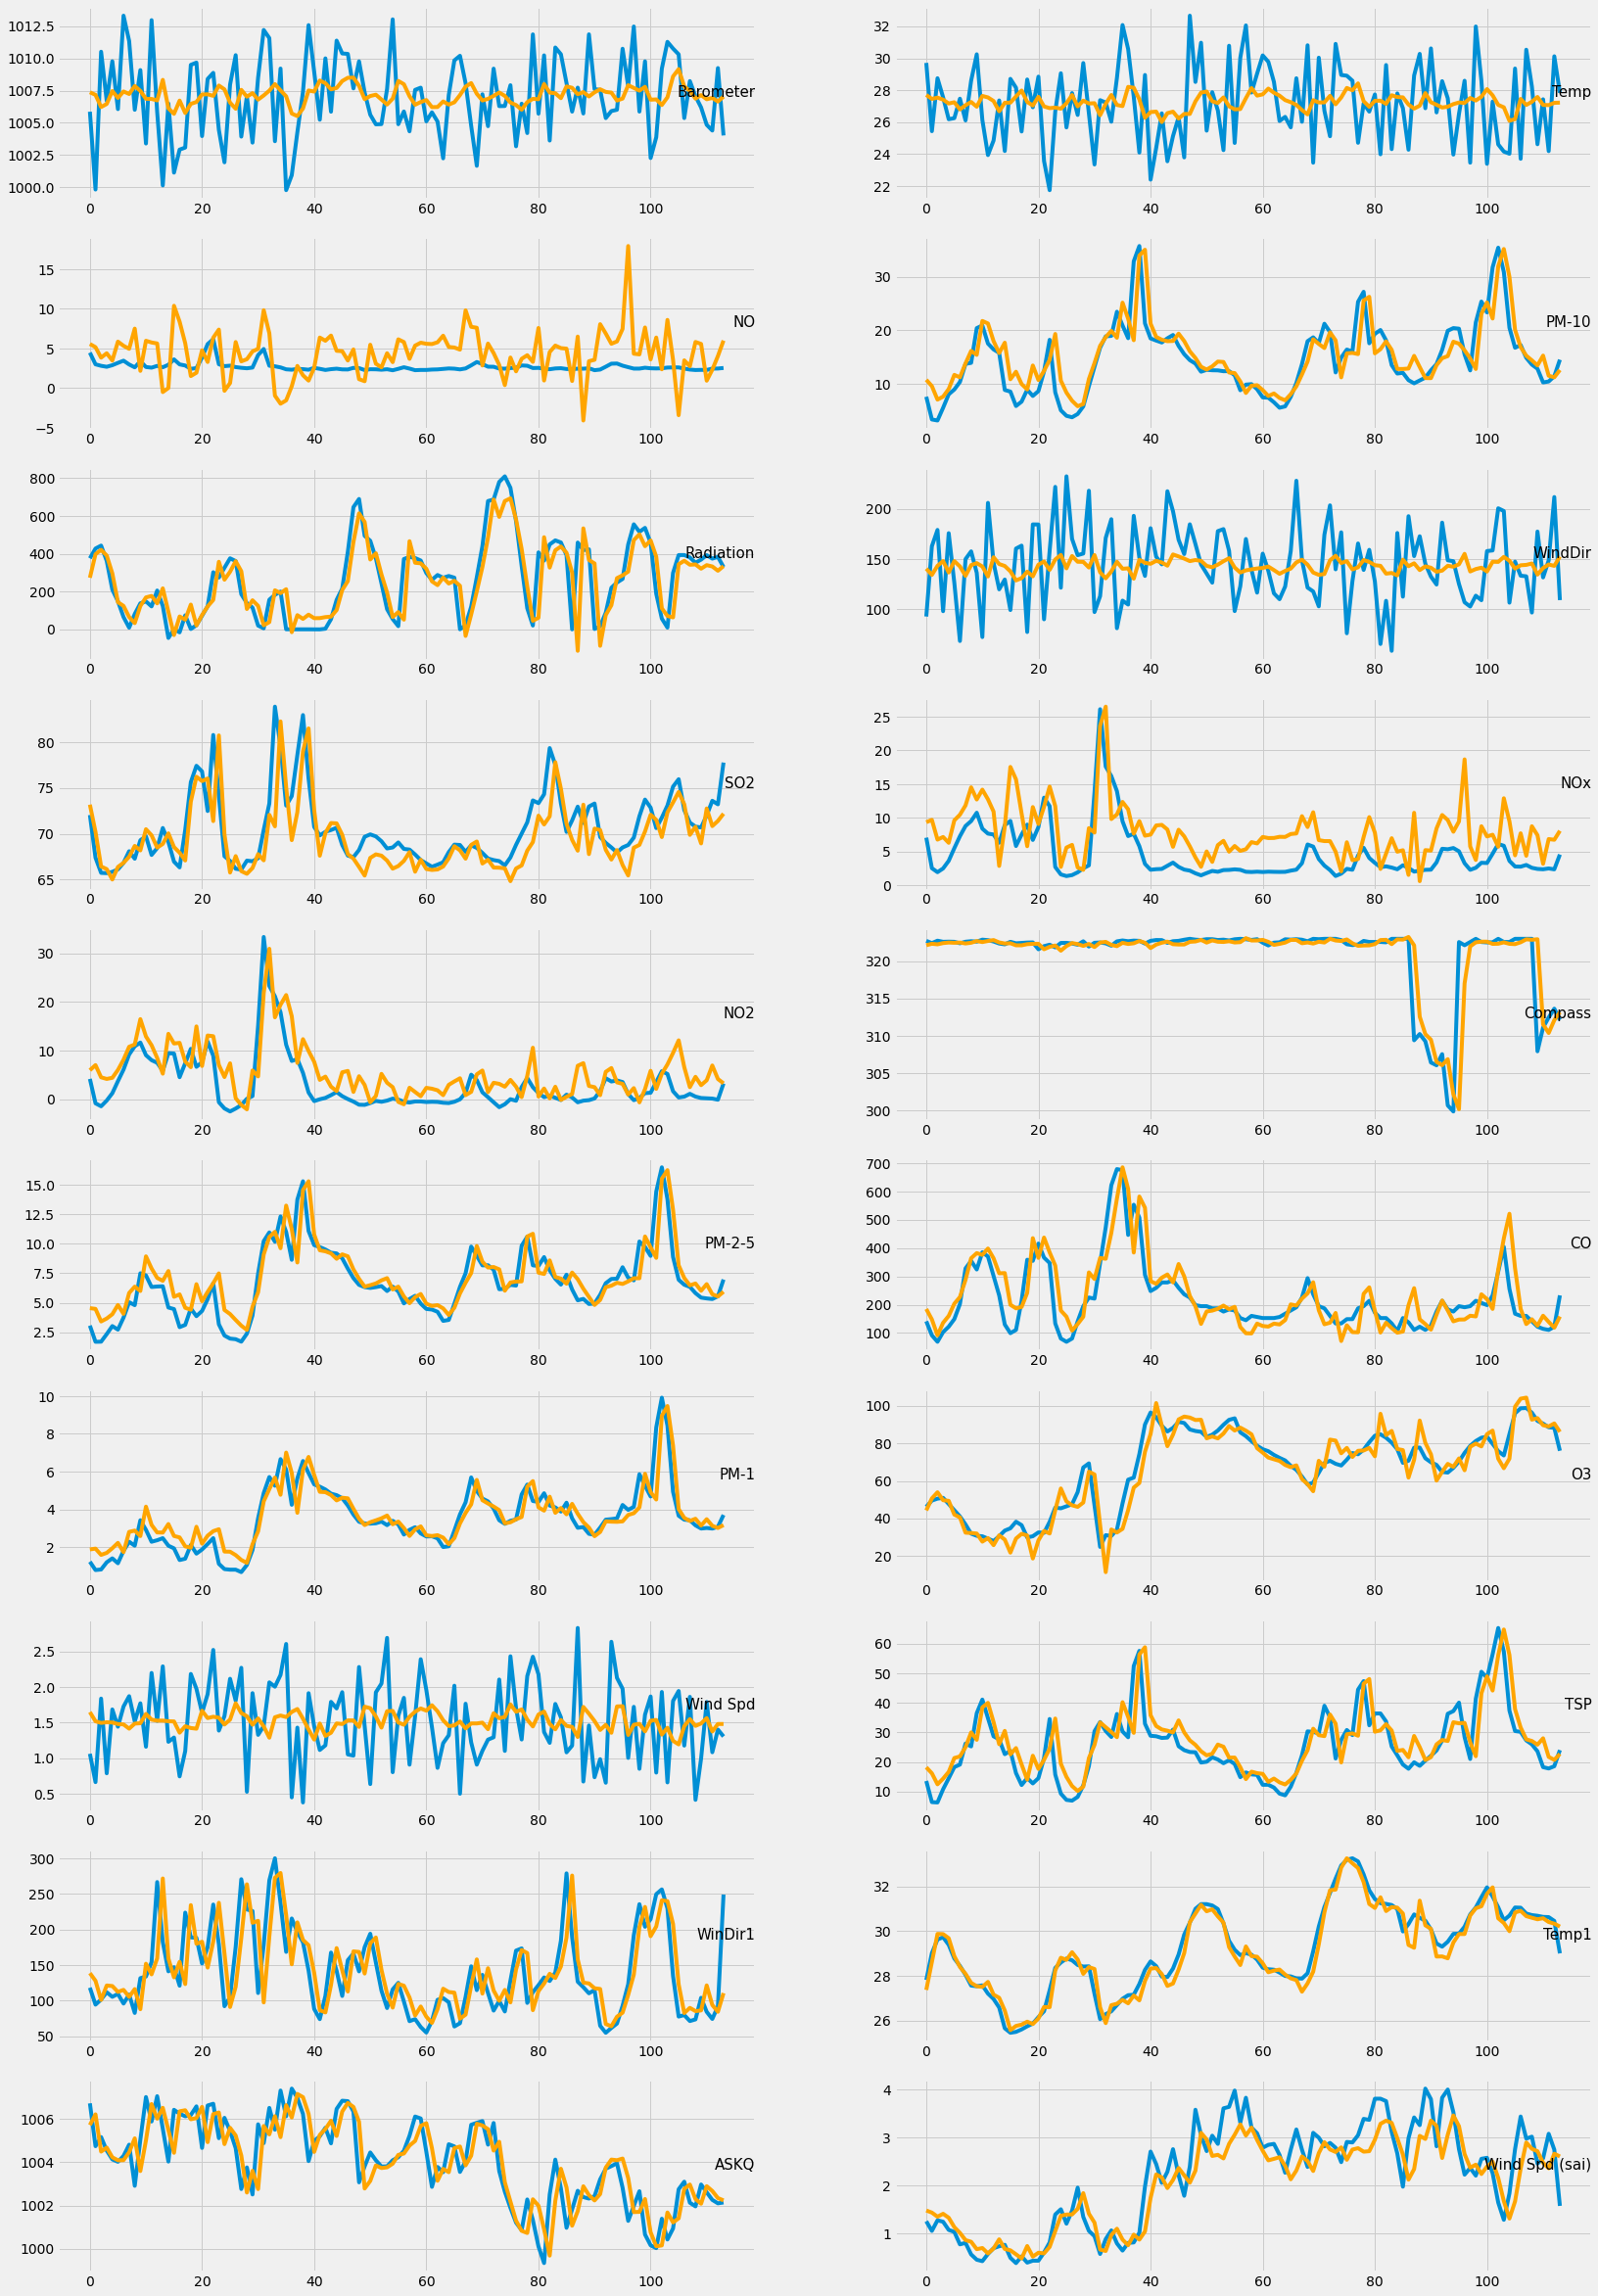
\includegraphics[width=.95\textwidth]{figures/VAR_test.png}
        \caption[Kết quả dự đoán so với tập test]{Kết quả dự đoán so với tập test}
    \end{figure}

    %\item Kết quả dự đoán 48 giờ sau đó
    %\begin{figure}[H]
    %    \centering
    %    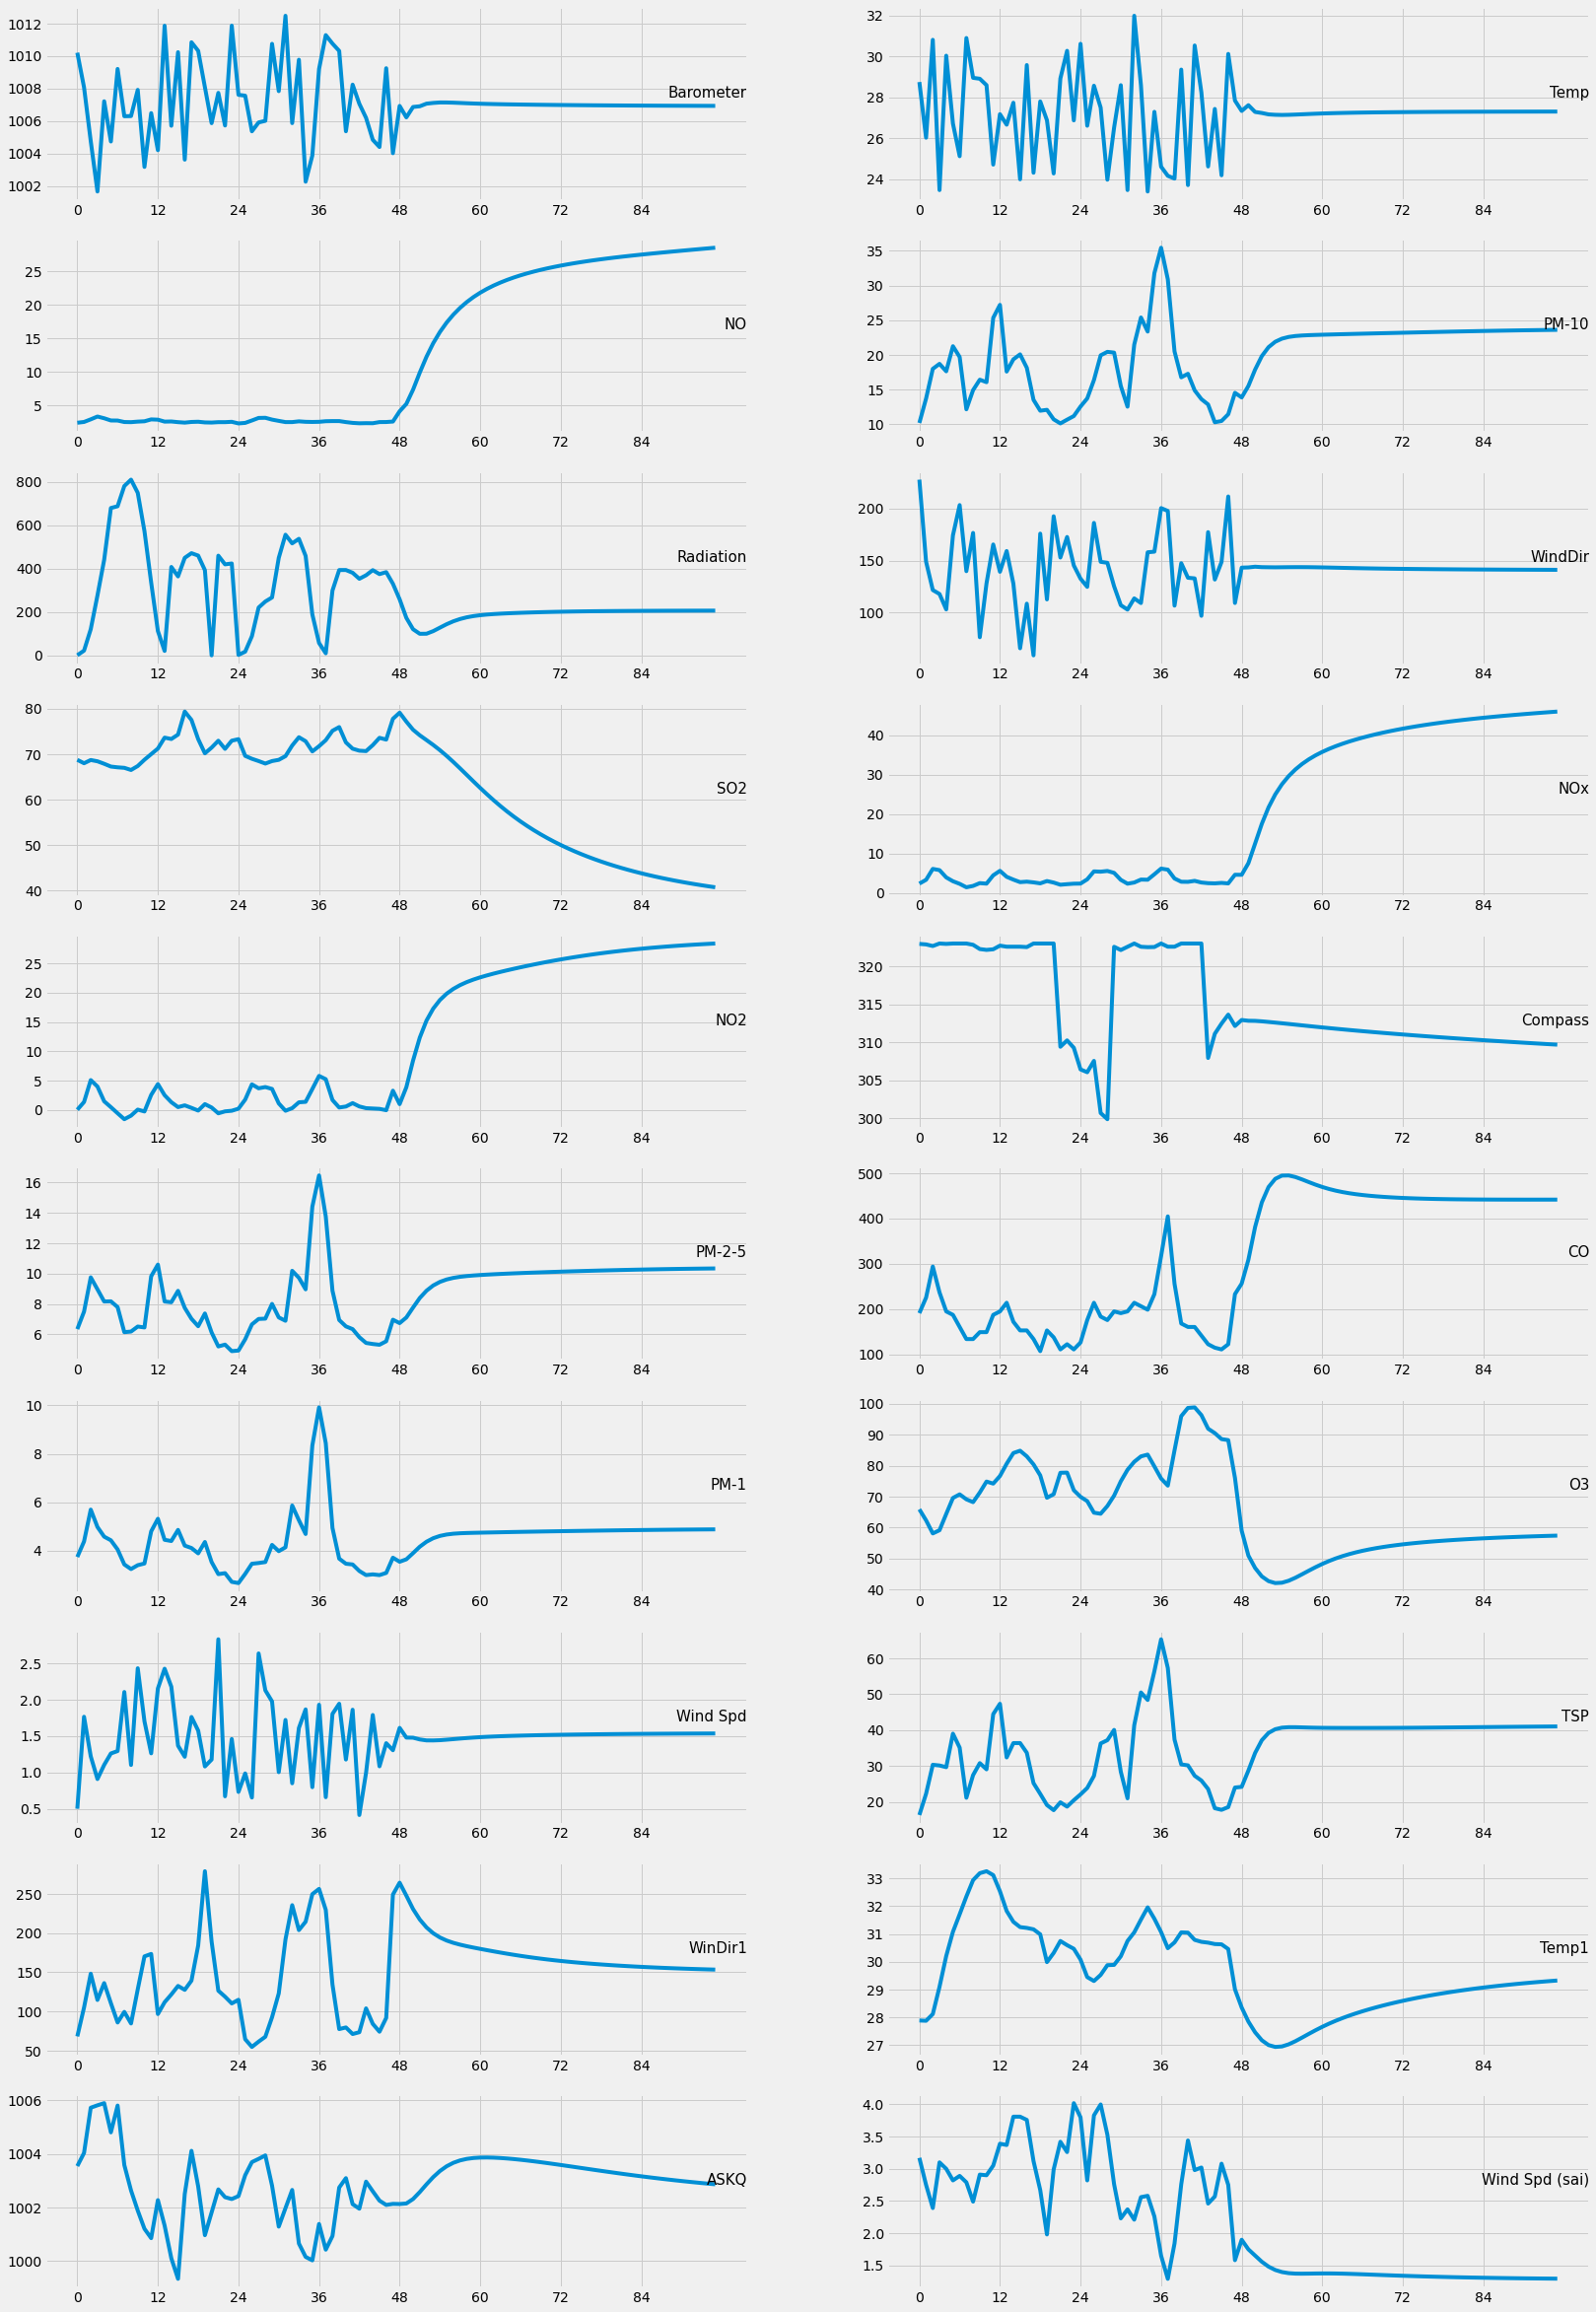
\includegraphics[width=.95\textwidth]{figures/VAR_predic.png}
    %    \caption[Kết quả dự đoán 48 giờ sau đó]{Kết quả dự đoán 48h sau đó}
    %\end{figure}
    %Hình ảnh trên biểu diễn các đồ thị của các cột với dữ liệu 48 giờ cuối của bộ dữ liệu và 48 giờ được dự đoán sau đó.
\end{enumerate}

Nhận xét:
\begin{itemize}
    \item Sau khi huấn luyện qua nhiều lần, thì giá trị MSE của mô hình VARMAX này vẫn khá cao.

    \item Tuy nhiên kết quả dự đoán so với kết quả test khá khớp với nhau trừ một số cột dữ liệu biến động mạnh.

    %\item Đồ thị kết quả dự đoán sau 48 giờ khá ổn định so với 48 giờ trước đó.

    \item Mô hình vẫn cần cải thiện để phù hợp với bộ dữ liệu hơn nữa.
\end{itemize}

\noindent \textbf{Nhận xét chung}: Với các kết quả thu được từ hai mô hình đã thử nghiệm LSTM và VARMAX trên, nhận thấy mô hình VARMAX là phù hợp với bộ dữ liệu hơn.